% Options for packages loaded elsewhere
\PassOptionsToPackage{unicode}{hyperref}
\PassOptionsToPackage{hyphens}{url}
\PassOptionsToPackage{dvipsnames,svgnames,x11names}{xcolor}
%
\documentclass[
  letterpaper,
  DIV=11,
  numbers=noendperiod]{scrartcl}

\usepackage{amsmath,amssymb}
\usepackage{iftex}
\ifPDFTeX
  \usepackage[T1]{fontenc}
  \usepackage[utf8]{inputenc}
  \usepackage{textcomp} % provide euro and other symbols
\else % if luatex or xetex
  \usepackage{unicode-math}
  \defaultfontfeatures{Scale=MatchLowercase}
  \defaultfontfeatures[\rmfamily]{Ligatures=TeX,Scale=1}
\fi
\usepackage{lmodern}
\ifPDFTeX\else  
    % xetex/luatex font selection
\fi
% Use upquote if available, for straight quotes in verbatim environments
\IfFileExists{upquote.sty}{\usepackage{upquote}}{}
\IfFileExists{microtype.sty}{% use microtype if available
  \usepackage[]{microtype}
  \UseMicrotypeSet[protrusion]{basicmath} % disable protrusion for tt fonts
}{}
\makeatletter
\@ifundefined{KOMAClassName}{% if non-KOMA class
  \IfFileExists{parskip.sty}{%
    \usepackage{parskip}
  }{% else
    \setlength{\parindent}{0pt}
    \setlength{\parskip}{6pt plus 2pt minus 1pt}}
}{% if KOMA class
  \KOMAoptions{parskip=half}}
\makeatother
\usepackage{xcolor}
\setlength{\emergencystretch}{3em} % prevent overfull lines
\setcounter{secnumdepth}{-\maxdimen} % remove section numbering
% Make \paragraph and \subparagraph free-standing
\ifx\paragraph\undefined\else
  \let\oldparagraph\paragraph
  \renewcommand{\paragraph}[1]{\oldparagraph{#1}\mbox{}}
\fi
\ifx\subparagraph\undefined\else
  \let\oldsubparagraph\subparagraph
  \renewcommand{\subparagraph}[1]{\oldsubparagraph{#1}\mbox{}}
\fi

\usepackage{color}
\usepackage{fancyvrb}
\newcommand{\VerbBar}{|}
\newcommand{\VERB}{\Verb[commandchars=\\\{\}]}
\DefineVerbatimEnvironment{Highlighting}{Verbatim}{commandchars=\\\{\}}
% Add ',fontsize=\small' for more characters per line
\usepackage{framed}
\definecolor{shadecolor}{RGB}{241,243,245}
\newenvironment{Shaded}{\begin{snugshade}}{\end{snugshade}}
\newcommand{\AlertTok}[1]{\textcolor[rgb]{0.68,0.00,0.00}{#1}}
\newcommand{\AnnotationTok}[1]{\textcolor[rgb]{0.37,0.37,0.37}{#1}}
\newcommand{\AttributeTok}[1]{\textcolor[rgb]{0.40,0.45,0.13}{#1}}
\newcommand{\BaseNTok}[1]{\textcolor[rgb]{0.68,0.00,0.00}{#1}}
\newcommand{\BuiltInTok}[1]{\textcolor[rgb]{0.00,0.23,0.31}{#1}}
\newcommand{\CharTok}[1]{\textcolor[rgb]{0.13,0.47,0.30}{#1}}
\newcommand{\CommentTok}[1]{\textcolor[rgb]{0.37,0.37,0.37}{#1}}
\newcommand{\CommentVarTok}[1]{\textcolor[rgb]{0.37,0.37,0.37}{\textit{#1}}}
\newcommand{\ConstantTok}[1]{\textcolor[rgb]{0.56,0.35,0.01}{#1}}
\newcommand{\ControlFlowTok}[1]{\textcolor[rgb]{0.00,0.23,0.31}{#1}}
\newcommand{\DataTypeTok}[1]{\textcolor[rgb]{0.68,0.00,0.00}{#1}}
\newcommand{\DecValTok}[1]{\textcolor[rgb]{0.68,0.00,0.00}{#1}}
\newcommand{\DocumentationTok}[1]{\textcolor[rgb]{0.37,0.37,0.37}{\textit{#1}}}
\newcommand{\ErrorTok}[1]{\textcolor[rgb]{0.68,0.00,0.00}{#1}}
\newcommand{\ExtensionTok}[1]{\textcolor[rgb]{0.00,0.23,0.31}{#1}}
\newcommand{\FloatTok}[1]{\textcolor[rgb]{0.68,0.00,0.00}{#1}}
\newcommand{\FunctionTok}[1]{\textcolor[rgb]{0.28,0.35,0.67}{#1}}
\newcommand{\ImportTok}[1]{\textcolor[rgb]{0.00,0.46,0.62}{#1}}
\newcommand{\InformationTok}[1]{\textcolor[rgb]{0.37,0.37,0.37}{#1}}
\newcommand{\KeywordTok}[1]{\textcolor[rgb]{0.00,0.23,0.31}{#1}}
\newcommand{\NormalTok}[1]{\textcolor[rgb]{0.00,0.23,0.31}{#1}}
\newcommand{\OperatorTok}[1]{\textcolor[rgb]{0.37,0.37,0.37}{#1}}
\newcommand{\OtherTok}[1]{\textcolor[rgb]{0.00,0.23,0.31}{#1}}
\newcommand{\PreprocessorTok}[1]{\textcolor[rgb]{0.68,0.00,0.00}{#1}}
\newcommand{\RegionMarkerTok}[1]{\textcolor[rgb]{0.00,0.23,0.31}{#1}}
\newcommand{\SpecialCharTok}[1]{\textcolor[rgb]{0.37,0.37,0.37}{#1}}
\newcommand{\SpecialStringTok}[1]{\textcolor[rgb]{0.13,0.47,0.30}{#1}}
\newcommand{\StringTok}[1]{\textcolor[rgb]{0.13,0.47,0.30}{#1}}
\newcommand{\VariableTok}[1]{\textcolor[rgb]{0.07,0.07,0.07}{#1}}
\newcommand{\VerbatimStringTok}[1]{\textcolor[rgb]{0.13,0.47,0.30}{#1}}
\newcommand{\WarningTok}[1]{\textcolor[rgb]{0.37,0.37,0.37}{\textit{#1}}}

\providecommand{\tightlist}{%
  \setlength{\itemsep}{0pt}\setlength{\parskip}{0pt}}\usepackage{longtable,booktabs,array}
\usepackage{calc} % for calculating minipage widths
% Correct order of tables after \paragraph or \subparagraph
\usepackage{etoolbox}
\makeatletter
\patchcmd\longtable{\par}{\if@noskipsec\mbox{}\fi\par}{}{}
\makeatother
% Allow footnotes in longtable head/foot
\IfFileExists{footnotehyper.sty}{\usepackage{footnotehyper}}{\usepackage{footnote}}
\makesavenoteenv{longtable}
\usepackage{graphicx}
\makeatletter
\def\maxwidth{\ifdim\Gin@nat@width>\linewidth\linewidth\else\Gin@nat@width\fi}
\def\maxheight{\ifdim\Gin@nat@height>\textheight\textheight\else\Gin@nat@height\fi}
\makeatother
% Scale images if necessary, so that they will not overflow the page
% margins by default, and it is still possible to overwrite the defaults
% using explicit options in \includegraphics[width, height, ...]{}
\setkeys{Gin}{width=\maxwidth,height=\maxheight,keepaspectratio}
% Set default figure placement to htbp
\makeatletter
\def\fps@figure{htbp}
\makeatother

\KOMAoption{captions}{tableheading}
\makeatletter
\@ifpackageloaded{tcolorbox}{}{\usepackage[skins,breakable]{tcolorbox}}
\@ifpackageloaded{fontawesome5}{}{\usepackage{fontawesome5}}
\definecolor{quarto-callout-color}{HTML}{909090}
\definecolor{quarto-callout-note-color}{HTML}{0758E5}
\definecolor{quarto-callout-important-color}{HTML}{CC1914}
\definecolor{quarto-callout-warning-color}{HTML}{EB9113}
\definecolor{quarto-callout-tip-color}{HTML}{00A047}
\definecolor{quarto-callout-caution-color}{HTML}{FC5300}
\definecolor{quarto-callout-color-frame}{HTML}{acacac}
\definecolor{quarto-callout-note-color-frame}{HTML}{4582ec}
\definecolor{quarto-callout-important-color-frame}{HTML}{d9534f}
\definecolor{quarto-callout-warning-color-frame}{HTML}{f0ad4e}
\definecolor{quarto-callout-tip-color-frame}{HTML}{02b875}
\definecolor{quarto-callout-caution-color-frame}{HTML}{fd7e14}
\makeatother
\makeatletter
\@ifpackageloaded{caption}{}{\usepackage{caption}}
\AtBeginDocument{%
\ifdefined\contentsname
  \renewcommand*\contentsname{Table of contents}
\else
  \newcommand\contentsname{Table of contents}
\fi
\ifdefined\listfigurename
  \renewcommand*\listfigurename{List of Figures}
\else
  \newcommand\listfigurename{List of Figures}
\fi
\ifdefined\listtablename
  \renewcommand*\listtablename{List of Tables}
\else
  \newcommand\listtablename{List of Tables}
\fi
\ifdefined\figurename
  \renewcommand*\figurename{Figure}
\else
  \newcommand\figurename{Figure}
\fi
\ifdefined\tablename
  \renewcommand*\tablename{Table}
\else
  \newcommand\tablename{Table}
\fi
}
\@ifpackageloaded{float}{}{\usepackage{float}}
\floatstyle{ruled}
\@ifundefined{c@chapter}{\newfloat{codelisting}{h}{lop}}{\newfloat{codelisting}{h}{lop}[chapter]}
\floatname{codelisting}{Listing}
\newcommand*\listoflistings{\listof{codelisting}{List of Listings}}
\makeatother
\makeatletter
\makeatother
\makeatletter
\@ifpackageloaded{caption}{}{\usepackage{caption}}
\@ifpackageloaded{subcaption}{}{\usepackage{subcaption}}
\makeatother
\ifLuaTeX
  \usepackage{selnolig}  % disable illegal ligatures
\fi
\usepackage{bookmark}

\IfFileExists{xurl.sty}{\usepackage{xurl}}{} % add URL line breaks if available
\urlstyle{same} % disable monospaced font for URLs
\hypersetup{
  pdftitle={Structured populations},
  pdfauthor={Henri Kauhanen},
  colorlinks=true,
  linkcolor={blue},
  filecolor={Maroon},
  citecolor={Blue},
  urlcolor={Blue},
  pdfcreator={LaTeX via pandoc}}

\title{Structured populations}
\usepackage{etoolbox}
\makeatletter
\providecommand{\subtitle}[1]{% add subtitle to \maketitle
  \apptocmd{\@title}{\par {\large #1 \par}}{}{}
}
\makeatother
\subtitle{Agent-based modelling, Konstanz, 2024}
\author{Henri Kauhanen}
\date{14 May 2024}

\begin{document}
\maketitle

\subsection{Plan}\label{plan}

\begin{itemize}
\tightlist
\item
  So far, we have had agents interacting randomly
\item
  We did this by:

  \begin{itemize}
  \tightlist
  \item
    initializing a population, \texttt{pop}, using an array
    comprehension
  \item
    using \texttt{rand(pop)} to sample random agents
  \item
    using our own function \texttt{interact!} to make two agents
    interact
  \end{itemize}
\end{itemize}

\begin{itemize}
\tightlist
\item
  Today: using \emph{Agents.jl} to work with \textbf{structured
  populations}
\end{itemize}

\subsection{Positional vs.~keyword
arguments}\label{positional-vs.-keyword-arguments}

\begin{itemize}
\tightlist
\item
  First, though, a technical remark about function arguments
\item
  We've seen function calls like this:
\end{itemize}

\begin{Shaded}
\begin{Highlighting}[]
\FunctionTok{plot}\NormalTok{(}\FloatTok{1}\OperatorTok{:}\FloatTok{100}\NormalTok{, (}\FloatTok{1}\OperatorTok{:}\FloatTok{100}\NormalTok{) }\OperatorTok{.\^{}} \FloatTok{2}\NormalTok{, seriestype }\OperatorTok{=} \OperatorTok{:}\NormalTok{scatter, color }\OperatorTok{=} \OperatorTok{:}\NormalTok{blue)}
\end{Highlighting}
\end{Shaded}

\begin{itemize}
\tightlist
\item
  Here,

  \begin{itemize}
  \tightlist
  \item
    \texttt{1:100} and \texttt{(1:100)\ .\^{}\ 2} are \textbf{positional
    arguments}
  \item
    \texttt{seriestype\ =\ :scatter} and \texttt{color\ =\ :blue} are
    \textbf{keyword arguments}
  \end{itemize}
\item
  You can swap the order of the latter but not of the former
\end{itemize}

\begin{itemize}
\tightlist
\item
  To create keyword arguments in your own function, you separate the
  list of keyword and positional arguments with a semicolon
  (\texttt{;}):
\end{itemize}

\begin{Shaded}
\begin{Highlighting}[]
\KeywordTok{function} \FunctionTok{my\_fun}\NormalTok{(pos1, pos2; keyword1, keyword2)}
  \OperatorTok{...}
\KeywordTok{end}
\end{Highlighting}
\end{Shaded}

\begin{itemize}
\tightlist
\item
  If you don't want any positional arguments, you have to write the
  following!
\end{itemize}

\begin{Shaded}
\begin{Highlighting}[]
\KeywordTok{function} \FunctionTok{my\_fun}\NormalTok{(; keyword1, keyword2)}
  \OperatorTok{...}
\KeywordTok{end}
\end{Highlighting}
\end{Shaded}

\begin{itemize}
\tightlist
\item
  Keyword (but not positional) arguments can have default values:
\end{itemize}

\begin{Shaded}
\begin{Highlighting}[]
\KeywordTok{function} \FunctionTok{my\_fun}\NormalTok{(; firstname }\OperatorTok{=} \StringTok{"John"}\NormalTok{, lastname)}
  \FunctionTok{println}\NormalTok{(firstname }\OperatorTok{*} \StringTok{" "} \OperatorTok{*}\NormalTok{ lastname)}
\KeywordTok{end}

\FunctionTok{my\_fun}\NormalTok{(firstname }\OperatorTok{=} \StringTok{"Jane"}\NormalTok{, lastname }\OperatorTok{=} \StringTok{"Doe"}\NormalTok{)}
\FunctionTok{my\_fun}\NormalTok{(lastname }\OperatorTok{=} \StringTok{"Doe"}\NormalTok{)}
\end{Highlighting}
\end{Shaded}

\begin{verbatim}
Jane Doe
John Doe
\end{verbatim}

\subsection{Structured populations}\label{structured-populations}

\begin{itemize}
\tightlist
\item
  I define a population to be \textbf{structured} whenever speakers do
  not interact fully at random
\end{itemize}

\begin{itemize}
\tightlist
\item
  Formally:

  \begin{itemize}
  \tightlist
  \item
    let \(P(X)\) = probability of sampling agent \(X\) for an
    interaction
  \item
    let \(P(Y \mid X)\) = (conditional) probability of sampling agent
    \(Y\), given that \(X\) was already sampled
  \item
    then population is \textbf{structured} if \(P(Y \mid X) = P(Y)\)
  \end{itemize}
\end{itemize}

\begin{itemize}
\tightlist
\item
  Example: \(P(\text{D. Trump} \mid \text{Henri}) = 0\) even though
  \(P(\text{D. Trump}) > 0\)
\end{itemize}

\subsection{Implementation}\label{implementation}

\begin{itemize}
\tightlist
\item
  It would be possible for us to write code for structured populations
  from scratch
\item
  However, this would be more of an exercise in programming than in
  ABMs\ldots{}
\item
  We're better off, here, using code written by other people
\item
  Enter the
  \href{https://juliadynamics.github.io/Agents.jl/stable/}{\emph{Agents.jl}}
  package, an ecosystem/framework for ABMs in Julia
\item
  You should already have \emph{Agents} installed. If not, now's the
  time to:
\end{itemize}

\begin{Shaded}
\begin{Highlighting}[]
\ImportTok{using} \BuiltInTok{Pkg}
\BuiltInTok{Pkg}\NormalTok{.}\FunctionTok{add}\NormalTok{(}\StringTok{"Agents"}\NormalTok{)}
\end{Highlighting}
\end{Shaded}

\subsection{Agents.jl basic steps}\label{agents.jl-basic-steps}

\begin{enumerate}
\def\labelenumi{\arabic{enumi}.}
\tightlist
\item
  Decide on model space (e.g.~social network)
\item
  Define agent type(s) (using special \texttt{@agent} keyword)
\item
  Define rules that evolve the model
\item
  Initialize your model with \texttt{AgentBasedModel}
\item
  Evolve, visualize and collect data
\end{enumerate}

\begin{itemize}
\tightlist
\item
  This may seem intimidating at first, but is really quite simple!
\item
  Let's walk through an example: variational learners in space
\end{itemize}

\subsection{Grid space}\label{grid-space}

\begin{itemize}
\tightlist
\item
  For this, we will reuse (with some modifications) our code for
  variational learners
\item
  And assume that individual learners/agents occupy the nodes of a
  \textbf{grid}, also known as a two-dimensional regular lattice:
\end{itemize}

\includegraphics[width=\textwidth,height=2.08333in]{../img/grid.png}

\begin{itemize}
\tightlist
\item
  Point: interactions \textbf{only} occur along links in this grid
\end{itemize}

\subsection{Grid space: implementation}\label{grid-space-implementation}

\begin{itemize}
\tightlist
\item
  To implement this in Julia with Agents.jl:
\end{itemize}

\begin{Shaded}
\begin{Highlighting}[]
\NormalTok{dims }\OperatorTok{=}\NormalTok{ (}\FloatTok{50}\NormalTok{, }\FloatTok{50}\NormalTok{)}
\NormalTok{space }\OperatorTok{=} \FunctionTok{GridSpaceSingle}\NormalTok{(dims)}
\end{Highlighting}
\end{Shaded}

\begin{itemize}
\tightlist
\item
  \texttt{(50,\ 50)} is a data structure known as a \textbf{tuple}
\item
  \texttt{GridSpaceSingle} comes from Agents.jl and defines a grid space
  in which each node can carry at most one agent (hence,
  \texttt{Single})
\end{itemize}

\begin{tcolorbox}[enhanced jigsaw, breakable, title=\textcolor{quarto-callout-note-color}{\faInfo}\hspace{0.5em}{Tuples and arrays}, bottomrule=.15mm, coltitle=black, toprule=.15mm, titlerule=0mm, colframe=quarto-callout-note-color-frame, toptitle=1mm, opacityback=0, colbacktitle=quarto-callout-note-color!10!white, rightrule=.15mm, bottomtitle=1mm, arc=.35mm, leftrule=.75mm, opacitybacktitle=0.6, colback=white, left=2mm]

Tuples are similar to arrays. However, there are important differences.
The most important of them is that arrays are mutable (the values of
their elements can be changed after creation), while tuples are never
mutable. Compare:

\begin{Shaded}
\begin{Highlighting}[]
\NormalTok{arr }\OperatorTok{=}\NormalTok{ [}\FloatTok{10}\NormalTok{,}\FloatTok{20}\NormalTok{]}
\NormalTok{tup }\OperatorTok{=}\NormalTok{ (}\FloatTok{10}\NormalTok{,}\FloatTok{20}\NormalTok{)}
\NormalTok{arr[}\FloatTok{1}\NormalTok{] }\OperatorTok{=} \FloatTok{30}   \CommentTok{\# arr is now [30,20]}
\NormalTok{tup[}\FloatTok{1}\NormalTok{] }\OperatorTok{=} \FloatTok{30}   \CommentTok{\# throws an error}
\end{Highlighting}
\end{Shaded}

The developers of Agents.jl have decided that the argument of
\texttt{GridSpaceSingle} has to be a tuple (this decision makes sense in
this case---as an immutable type, a tuple is more efficient than an
array of similar size).

\textbf{If you are running into errors trying to initialize a
\texttt{GridSpaceSingle}, the problem is probably that you are trying to
pass it the wrong type of argument.} Compare:

\begin{Shaded}
\begin{Highlighting}[]
\FunctionTok{GridSpaceSingle}\NormalTok{([}\FloatTok{50}\NormalTok{, }\FloatTok{50}\NormalTok{])   }\CommentTok{\# trying to pass array; error}
\FunctionTok{GridSpaceSingle}\NormalTok{(}\FloatTok{50}\NormalTok{, }\FloatTok{50}\NormalTok{)     }\CommentTok{\# trying to pass two separate numbers; error}
\FunctionTok{GridSpaceSingle}\NormalTok{((}\FloatTok{50}\NormalTok{, }\FloatTok{50}\NormalTok{))   }\CommentTok{\# passing a tuple; works}
\end{Highlighting}
\end{Shaded}

\end{tcolorbox}

\subsection{Agent redefinition}\label{agent-redefinition}

\begin{itemize}
\tightlist
\item
  To make use of the machinery provided by \emph{Agents.jl}, we replace:
\end{itemize}

\begin{Shaded}
\begin{Highlighting}[]
\KeywordTok{mutable struct}\NormalTok{ VariationalLearner}
\NormalTok{  p}\OperatorTok{::}\DataTypeTok{Float64}
\NormalTok{  gamma}\OperatorTok{::}\DataTypeTok{Float64}
\NormalTok{  P1}\OperatorTok{::}\DataTypeTok{Float64}
\NormalTok{  P2}\OperatorTok{::}\DataTypeTok{Float64}
\KeywordTok{end}
\end{Highlighting}
\end{Shaded}

\begin{itemize}
\tightlist
\item
  with this:
\end{itemize}

\begin{Shaded}
\begin{Highlighting}[]
\PreprocessorTok{@agent} \KeywordTok{struct} \FunctionTok{VariationalLearner}\NormalTok{(GridAgent\{}\FloatTok{2}\NormalTok{\})}
\NormalTok{  p}\OperatorTok{::}\DataTypeTok{Float64}
\NormalTok{  gamma}\OperatorTok{::}\DataTypeTok{Float64}
\NormalTok{  P1}\OperatorTok{::}\DataTypeTok{Float64}
\NormalTok{  P2}\OperatorTok{::}\DataTypeTok{Float64}
\KeywordTok{end}
\end{Highlighting}
\end{Shaded}

\begin{itemize}
\tightlist
\item
  \texttt{@agent} is a special ``macro'' (more on these later) that
  introduces all agents in Agents.jl
\item
  \texttt{GridAgent\{2\}} instructs Agents.jl that this agent is to be
  used in a 2-dimensional grid space
\end{itemize}

\subsection{Stepping rule}\label{stepping-rule}

\begin{itemize}
\tightlist
\item
  We next need a function that evolves i.e.~\textbf{steps} the model
\item
  This is a function that takes a single agent and the model as
  arguments
\item
  We can make use of the \texttt{interact!} function we have already
  written:
\end{itemize}

\begin{Shaded}
\begin{Highlighting}[]
\KeywordTok{function} \FunctionTok{VL\_step!}\NormalTok{(agent, model)}
\NormalTok{  interlocutor }\OperatorTok{=} \FunctionTok{random\_nearby\_agent}\NormalTok{(agent, model)}
  \FunctionTok{interact!}\NormalTok{(interlocutor, agent)}
\KeywordTok{end}
\end{Highlighting}
\end{Shaded}

\subsection{Model initialization}\label{model-initialization}

\begin{itemize}
\tightlist
\item
  We now have all the ingredients we need to initialize the ABM:
\end{itemize}

\begin{Shaded}
\begin{Highlighting}[]
\NormalTok{model }\OperatorTok{=} \FunctionTok{StandardABM}\NormalTok{(VariationalLearner, space; }
\NormalTok{                    agent\_step! }\OperatorTok{=}\NormalTok{ VL\_step!)}
\end{Highlighting}
\end{Shaded}

\begin{verbatim}
StandardABM with 0 agents of type VariationalLearner
 agents container: Dict
 space: GridSpaceSingle with size (50, 50), metric=chebyshev, periodic=true
 scheduler: fastest
\end{verbatim}

In the above function call, you \textbf{cannot} write
\texttt{agent\_step!=VL\_step!} (i.e.~without spaces around the
\texttt{=} sign). This is because, if you do so, Julia parses this as
\texttt{agent\_step\ !=\ VL\_step!}, which is not what we want.

In other words, when using keyword arguments with exclamation points in
their names, make it a habit to separate the equals sign with spaces.

\begin{itemize}
\tightlist
\item
  This creates a sort of an ``empty'' container (it has no agents yet).
  To add agents, we call:
\end{itemize}

\begin{Shaded}
\begin{Highlighting}[]
\FunctionTok{add\_agent\_single!}\NormalTok{(model; p }\OperatorTok{=} \FloatTok{0.1}\NormalTok{, gamma }\OperatorTok{=} \FloatTok{0.01}\NormalTok{, }
\NormalTok{                  P1 }\OperatorTok{=} \FloatTok{0.4}\NormalTok{, P2 }\OperatorTok{=} \FloatTok{0.1}\NormalTok{)}
\end{Highlighting}
\end{Shaded}

\begin{verbatim}
VariationalLearner(1, (4, 27), 0.1, 0.01, 0.4, 0.1)
\end{verbatim}

\begin{itemize}
\tightlist
\item
  Note: the values of the agent's internal fields (\texttt{p},
  \texttt{gamma} etc.) are specified as keyword arguments!
\end{itemize}

\begin{itemize}
\tightlist
\item
  We have a space of 50 x 50 = 2,500 nodes
\item
  Let's add 2,499 more agents:
\end{itemize}

\begin{Shaded}
\begin{Highlighting}[]
\ControlFlowTok{for}\NormalTok{ i }\KeywordTok{in} \FloatTok{1}\OperatorTok{:}\FloatTok{2499}
  \FunctionTok{add\_agent\_single!}\NormalTok{(model; p }\OperatorTok{=} \FloatTok{0.1}\NormalTok{, gamma }\OperatorTok{=} \FloatTok{0.01}\NormalTok{, }
\NormalTok{                    P1 }\OperatorTok{=} \FloatTok{0.4}\NormalTok{, P2 }\OperatorTok{=} \FloatTok{0.1}\NormalTok{)}
\ControlFlowTok{end}
\end{Highlighting}
\end{Shaded}

\begin{itemize}
\tightlist
\item
  Check number of agents:
\end{itemize}

\begin{Shaded}
\begin{Highlighting}[]
\FunctionTok{nagents}\NormalTok{(model)}
\end{Highlighting}
\end{Shaded}

\begin{verbatim}
2500
\end{verbatim}

\subsection{Stepping the model}\label{stepping-the-model}

\begin{itemize}
\tightlist
\item
  Stepping the model is now easy:
\end{itemize}

\begin{Shaded}
\begin{Highlighting}[]
\FunctionTok{step!}\NormalTok{(model)}
\end{Highlighting}
\end{Shaded}

\begin{verbatim}
StandardABM with 2500 agents of type VariationalLearner
 agents container: Dict
 space: GridSpaceSingle with size (50, 50), metric=chebyshev, periodic=true
 scheduler: fastest
\end{verbatim}

\begin{itemize}
\tightlist
\item
  Or, for a desired number of steps:
\end{itemize}

\begin{Shaded}
\begin{Highlighting}[]
\FunctionTok{step!}\NormalTok{(model, }\FloatTok{10}\NormalTok{)}
\end{Highlighting}
\end{Shaded}

\begin{verbatim}
StandardABM with 2500 agents of type VariationalLearner
 agents container: Dict
 space: GridSpaceSingle with size (50, 50), metric=chebyshev, periodic=true
 scheduler: fastest
\end{verbatim}

\begin{tcolorbox}[enhanced jigsaw, breakable, title=\textcolor{quarto-callout-important-color}{\faExclamation}\hspace{0.5em}{Important}, bottomrule=.15mm, coltitle=black, toprule=.15mm, titlerule=0mm, colframe=quarto-callout-important-color-frame, toptitle=1mm, opacityback=0, colbacktitle=quarto-callout-important-color!10!white, rightrule=.15mm, bottomtitle=1mm, arc=.35mm, leftrule=.75mm, opacitybacktitle=0.6, colback=white, left=2mm]

Stepping in Agents.jl is controlled by a so-called \textbf{scheduler}.
You can decide which scheduler to use when initializing your model; for
now, we will stick to the default scheduler.

This is important to know: when the default scheduler steps a model,
\textbf{every} agent gets updated. In the case of our model, this means
that every agent undergoes exactly one interaction as the ``listening''
party, i.e.~every agent gets to learn from exactly one interaction
during one time step.

\end{tcolorbox}

\subsection{Plotting the population}\label{plotting-the-population}

\begin{itemize}
\tightlist
\item
  With Agents.jl, we also have access to a number of functions that can
  be used for purposes of visualization
\item
  \texttt{abmplot(model)} plots \texttt{model} in its current state. It
  has \textbf{two} return values:

  \begin{itemize}
  \tightlist
  \item
    the first one is the plot itself
  \item
    the second one contains metadata which we usually don't need to care
    about
  \end{itemize}
\item
  To actually see the plot, you have to call the first return value
  explicitly:
\end{itemize}

\begin{Shaded}
\begin{Highlighting}[]
\NormalTok{fig, meta }\OperatorTok{=} \FunctionTok{abmplot}\NormalTok{(model)}
\NormalTok{fig}
\end{Highlighting}
\end{Shaded}

\begin{verbatim}
┌ Warning: Found `resolution` in the theme when creating a `Scene`. The `resolution` keyword for `Scene`s and `Figure`s has been deprecated. Use `Figure(; size = ...` or `Scene(; size = ...)` instead, which better reflects that this is a unitless size and not a pixel resolution. The key could also come from `set_theme!` calls or related theming functions.
└ @ Makie ~/.julia/packages/Makie/iRM0c/src/scenes.jl:220
\end{verbatim}

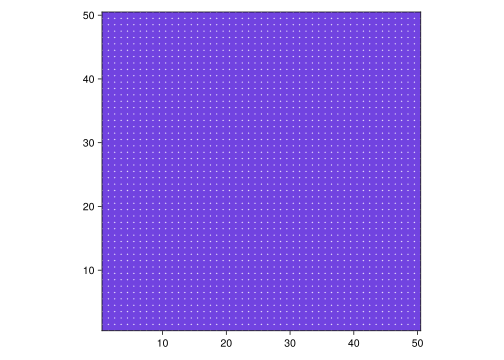
\includegraphics{networks_files/figure-pdf/cell-24-output-2.png}

\begin{itemize}
\tightlist
\item
  So all we get is a purple square\ldots{} what gives?
\item
  The problem is that we haven't yet instructed \texttt{abmplot}
  \textbf{how} we want our model to be visualized
\item
  We could in principle be interested in plotting various kinds of
  things
\item
  For our model here, it makes sense to plot the value of \texttt{p},
  i.e.~each learner's internal ``grammatical state''
\item
  This is done with a function that maps an agent to its \texttt{p}
\end{itemize}

\begin{itemize}
\tightlist
\item
  In this case, the function is as simple as:
\end{itemize}

\begin{Shaded}
\begin{Highlighting}[]
\KeywordTok{function} \FunctionTok{getp}\NormalTok{(a)}
  \ControlFlowTok{return}\NormalTok{ a.p}
\KeywordTok{end}
\end{Highlighting}
\end{Shaded}

\begin{verbatim}
getp (generic function with 1 method)
\end{verbatim}

\begin{tcolorbox}[enhanced jigsaw, breakable, title=\textcolor{quarto-callout-tip-color}{\faLightbulb}\hspace{0.5em}{Tip}, bottomrule=.15mm, coltitle=black, toprule=.15mm, titlerule=0mm, colframe=quarto-callout-tip-color-frame, toptitle=1mm, opacityback=0, colbacktitle=quarto-callout-tip-color!10!white, rightrule=.15mm, bottomtitle=1mm, arc=.35mm, leftrule=.75mm, opacitybacktitle=0.6, colback=white, left=2mm]

Julia also allows one-liner function definitions. These are often useful
when defining very simple functions, like \texttt{getp}. The equivalent
one-liner definition here is:

\begin{Shaded}
\begin{Highlighting}[]
\FunctionTok{getp}\NormalTok{(a) }\OperatorTok{=}\NormalTok{ a.p}
\end{Highlighting}
\end{Shaded}

\begin{verbatim}
getp (generic function with 1 method)
\end{verbatim}

\end{tcolorbox}

\begin{itemize}
\tightlist
\item
  We now pass our \texttt{getp} function as the value of the
  \texttt{agent\_color} keyword argument to \texttt{abmplot}:
\end{itemize}

\begin{Shaded}
\begin{Highlighting}[]
\NormalTok{fig, meta }\OperatorTok{=} \FunctionTok{abmplot}\NormalTok{(model; agent\_color }\OperatorTok{=}\NormalTok{ getp)}
\NormalTok{fig}
\end{Highlighting}
\end{Shaded}

\begin{verbatim}
┌ Warning: Found `resolution` in the theme when creating a `Scene`. The `resolution` keyword for `Scene`s and `Figure`s has been deprecated. Use `Figure(; size = ...` or `Scene(; size = ...)` instead, which better reflects that this is a unitless size and not a pixel resolution. The key could also come from `set_theme!` calls or related theming functions.
└ @ Makie ~/.julia/packages/Makie/iRM0c/src/scenes.jl:220
\end{verbatim}

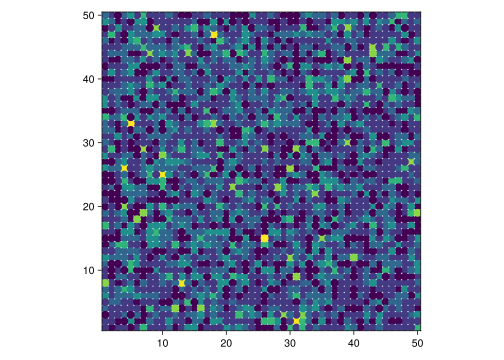
\includegraphics{networks_files/figure-pdf/cell-27-output-2.png}

\begin{itemize}
\tightlist
\item
  We can see how the population changes as we evolve the model further
  (the new \texttt{as} keyword argument specifies the size of the dots
  that represent the agents):
\end{itemize}

\begin{Shaded}
\begin{Highlighting}[]
\FunctionTok{step!}\NormalTok{(model, }\FloatTok{1000}\NormalTok{)}
\NormalTok{fig2, meta }\OperatorTok{=} \FunctionTok{abmplot}\NormalTok{(model; agent\_color }\OperatorTok{=}\NormalTok{ getp, as }\OperatorTok{=} \FloatTok{12}\NormalTok{)}
\NormalTok{fig2}
\end{Highlighting}
\end{Shaded}

\begin{verbatim}
┌ Warning: Found `resolution` in the theme when creating a `Scene`. The `resolution` keyword for `Scene`s and `Figure`s has been deprecated. Use `Figure(; size = ...` or `Scene(; size = ...)` instead, which better reflects that this is a unitless size and not a pixel resolution. The key could also come from `set_theme!` calls or related theming functions.
└ @ Makie ~/.julia/packages/Makie/iRM0c/src/scenes.jl:220
\end{verbatim}

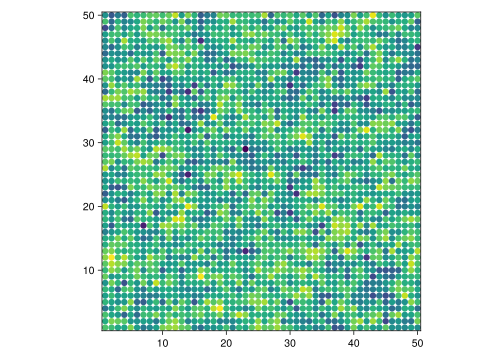
\includegraphics{networks_files/figure-pdf/cell-28-output-2.png}

\begin{itemize}
\tightlist
\item
  And further:
\end{itemize}

\begin{Shaded}
\begin{Highlighting}[]
\FunctionTok{step!}\NormalTok{(model, }\FloatTok{1000}\NormalTok{)}
\NormalTok{fig3, meta }\OperatorTok{=} \FunctionTok{abmplot}\NormalTok{(model; agent\_color }\OperatorTok{=}\NormalTok{ getp, as }\OperatorTok{=} \FloatTok{12}\NormalTok{)}
\NormalTok{fig3}
\end{Highlighting}
\end{Shaded}

\begin{verbatim}
┌ Warning: Found `resolution` in the theme when creating a `Scene`. The `resolution` keyword for `Scene`s and `Figure`s has been deprecated. Use `Figure(; size = ...` or `Scene(; size = ...)` instead, which better reflects that this is a unitless size and not a pixel resolution. The key could also come from `set_theme!` calls or related theming functions.
└ @ Makie ~/.julia/packages/Makie/iRM0c/src/scenes.jl:220
\end{verbatim}

\includegraphics{networks_files/figure-pdf/cell-29-output-2.png}

\begin{itemize}
\tightlist
\item
  Making an animation/video allows us to visualize the evolution
  dynamically
\item
  This is achieved with the \texttt{abmvideo} function
\end{itemize}

\begin{Shaded}
\begin{Highlighting}[]
\FunctionTok{abmvideo}\NormalTok{(}\StringTok{"vid.mp4"}\NormalTok{, model; agent\_color }\OperatorTok{=}\NormalTok{ getp, as }\OperatorTok{=} \FloatTok{12}\NormalTok{, }
\NormalTok{         frames }\OperatorTok{=} \FloatTok{100}\NormalTok{, framerate }\OperatorTok{=} \FloatTok{10}\NormalTok{)}
\end{Highlighting}
\end{Shaded}

\url{../videos/vid.mp4}

\subsection{A more interesting
example}\label{a-more-interesting-example}

\begin{itemize}
\tightlist
\item
  Above, we initialized the population so that everybody had
  \texttt{p\ =\ 0.1} in the beginning
\item
  What about the following: at time \(t=0\),

  \begin{itemize}
  \tightlist
  \item
    \textbf{three} people have \texttt{p\ =\ 1} (uses \(G_1\) all the
    time),
  \item
    every other person has \texttt{p\ =\ 0} (uses \(G_2\) all the time)?
  \end{itemize}
\item
  Will we see \(G_1\) spread across the population?
\item
  Let's try!
\end{itemize}

\begin{itemize}
\tightlist
\item
  We first reinitialize the model:
\end{itemize}

\begin{Shaded}
\begin{Highlighting}[]
\NormalTok{space2 }\OperatorTok{=} \FunctionTok{GridSpaceSingle}\NormalTok{((}\FloatTok{50}\NormalTok{, }\FloatTok{50}\NormalTok{))}
\NormalTok{model2 }\OperatorTok{=} \FunctionTok{StandardABM}\NormalTok{(VariationalLearner, space2;}
\NormalTok{                     agent\_step! }\OperatorTok{=}\NormalTok{ VL\_step!)}

\ControlFlowTok{for}\NormalTok{ i }\KeywordTok{in} \FloatTok{1}\OperatorTok{:}\FloatTok{3}
  \FunctionTok{add\_agent\_single!}\NormalTok{(model2; p }\OperatorTok{=} \FloatTok{1.0}\NormalTok{, gamma }\OperatorTok{=} \FloatTok{0.1}\NormalTok{, }
\NormalTok{                    P1 }\OperatorTok{=} \FloatTok{0.4}\NormalTok{, P2 }\OperatorTok{=} \FloatTok{0.1}\NormalTok{)}
\ControlFlowTok{end}

\ControlFlowTok{for}\NormalTok{ i }\KeywordTok{in} \FloatTok{4}\OperatorTok{:}\FloatTok{2500}
  \FunctionTok{add\_agent\_single!}\NormalTok{(model2; p }\OperatorTok{=} \FloatTok{0.0}\NormalTok{, gamma }\OperatorTok{=} \FloatTok{0.1}\NormalTok{, }
\NormalTok{                    P1 }\OperatorTok{=} \FloatTok{0.4}\NormalTok{, P2 }\OperatorTok{=} \FloatTok{0.1}\NormalTok{)}
\ControlFlowTok{end}
\end{Highlighting}
\end{Shaded}

\begin{tcolorbox}[enhanced jigsaw, breakable, title=\textcolor{quarto-callout-important-color}{\faExclamation}\hspace{0.5em}{Important}, bottomrule=.15mm, coltitle=black, toprule=.15mm, titlerule=0mm, colframe=quarto-callout-important-color-frame, toptitle=1mm, opacityback=0, colbacktitle=quarto-callout-important-color!10!white, rightrule=.15mm, bottomtitle=1mm, arc=.35mm, leftrule=.75mm, opacitybacktitle=0.6, colback=white, left=2mm]

Here it is important that we create a new space (I've called it
\texttt{space2}). Otherwise Agents.jl would try to add agents to our old
space, which is already full!

\end{tcolorbox}

\begin{itemize}
\tightlist
\item
  Visualize initial state of population:
\end{itemize}

\begin{Shaded}
\begin{Highlighting}[]
\NormalTok{fig, meta }\OperatorTok{=} \FunctionTok{abmplot}\NormalTok{(model2; agent\_color }\OperatorTok{=}\NormalTok{ getp, as }\OperatorTok{=} \FloatTok{12}\NormalTok{)}
\NormalTok{fig}
\end{Highlighting}
\end{Shaded}

\begin{verbatim}
┌ Warning: Found `resolution` in the theme when creating a `Scene`. The `resolution` keyword for `Scene`s and `Figure`s has been deprecated. Use `Figure(; size = ...` or `Scene(; size = ...)` instead, which better reflects that this is a unitless size and not a pixel resolution. The key could also come from `set_theme!` calls or related theming functions.
└ @ Makie ~/.julia/packages/Makie/iRM0c/src/scenes.jl:220
\end{verbatim}

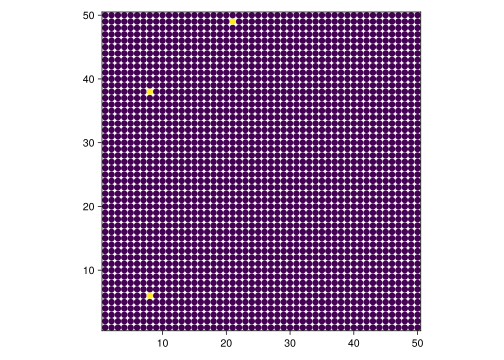
\includegraphics{networks_files/figure-pdf/cell-33-output-2.png}

\begin{itemize}
\tightlist
\item
  Animate for 1,000 iterations (every agent gets to learn 1,000 times):
\end{itemize}

\begin{Shaded}
\begin{Highlighting}[]
\FunctionTok{abmvideo}\NormalTok{(}\StringTok{"interesting.mp4"}\NormalTok{, model2; agent\_color }\OperatorTok{=}\NormalTok{ getp,}
\NormalTok{         as }\OperatorTok{=} \FloatTok{12}\NormalTok{, frames }\OperatorTok{=} \FloatTok{1000}\NormalTok{, framerate }\OperatorTok{=} \FloatTok{20}\NormalTok{)}
\end{Highlighting}
\end{Shaded}

\url{../videos/interesting.mp4}



\end{document}
